\section{Experiment 1}
\label{sec:exp1}
Experiment 1 trains and evaluates ANNs on the task to classify images of fruits and vegetables of 10 base types. The goal of the experiment is to try different network types in order to find the best configuration, i.e., the configuration with the lowest zero-one loss.

\subsection{Setup}
This experiment is carried out on a 64 bit machine running Fedora 32, with an Intel\textsuperscript{\textregistered} Core\texttrademark{} i7-2670QM CPU @ 2.20GHz and 6GByte of RAM. THe programming language used is Python 3.8\cite{python3}. Tensorflow2\cite{tensorflow2015-whitepaper}, with the Keras\cite{chollet2015keras} interface, is used to create, train and evaluate models. Numpy\cite{harris2020array} is used to store and manipulate data easily.

\textbf{Dataset.}
The dataset used is available on \href{https://www.kaggle.com/moltean/fruits}{kaggle.com/moltean/fruits}. It contains 90380 images of fruits and vegetables. Experiment 1 classifies images in 10 base types, namely "apple", "banana", "cherry", "grape", "peach", "pear", "pepper", "plum", "potato" and "tomato". Only the 43513 images that represents these fruit and vegetable types are considered. The images are 100x100px photos, already cropped to fit the subject perfectly.

The script \texttt{dataset\_1.py} is used to manage the dataset. This script performs 5 tasks. 1)It loads images from the dataset. 2)It labels images according to the folder they are in. If the name of the folder starts with one of the 10 labels, the label is attached to the image. Otherwise the image is discarded. 3)It resizes images according to a preferred size. 4)It generates Numpy's n-dimensional arrays containing image data and labels such that they can be easily fed to a machine learning model. The ndarray for image data is of type unsigned 8-bit integer and its shape is \texttt{(ni,is,is,3)}, where \texttt{ni} is the number of images, \texttt{is} is the image side length in pixel, and 3 is the number of channels (r,g,b). The ndarray for labels is of type unsigned 8-bit integer and its shape is \texttt{(ni,)}, where \texttt{ni} is the number of images. Arrays are created both for training and testing sets. 5)Finally, the script stores said arrays in binary format, so that it will load them faster at the next iteration, without having to go through the whole process again.

The script offers a simple interface, consisting of a single function \texttt{dataset(size)}, which takes care of all the aforementioned tasks in the background and returns the dataset, with images of the preferred size, ready to be used by a machine learning model. The \texttt{dataset(size)} function is declared as follows:
\begin{minted}{python}
def dataset(size):
    '''Return dataset with images of preferred size.
    If dataset already exists, it is loaded from disk,
    otherwise it is created from the image folder.'''
    files = (
        join(dataset_folder,f'x_train_{size}.npy'),
        join(dataset_folder,f'y_train_{size}.npy'),
        join(dataset_folder,f'x_test_{size}.npy'),
        join(dataset_folder,f'y_test_{size}.npy'))
    for f in files:
        if not isfile(f):
            ds = create_dataset(size)
            save_dataset(*ds,size)
            return ds
    return load_dataset(size)
\end{minted}

\textbf{Models.}
The models used differ in size, shape and type. The script \texttt{models.py} handles the creation of models according to certain parameters. The parameters supported are depth of the network, i.e., how many layers it has, width of the network, i.e., how many nodes are in each layer, type of network, i.e., DNN or CNN. Furthermore the script can handle different input and output sizes according to the needs.

The script offers a simple interface, consisting of a generator that yields models ready to be tested. The generator is called using the function \texttt{models(input\_size, output\_size)}. For this experiment, the generator is tuned to return 30 different networks. The number 30 is the result of the combination of 2 types of networks (DNN and CNN), 3 depths (1,2 or 3 layers), 5 widths (multiples of 32 in the case od DNN and multiples of 8 in the case of CNN).The \texttt{models(input\_size, output\_size)} function is coded as follows:
\begin{minted}{python}
def models(input_size,output_size):
    '''This generator returns models to testing in the experiment.'''
    #dense layers, different sizes
    for i in range(1,4):
        for j in range(1,6):
            yield dense(input_size,output_size,i,j*32),i,j*32,'dense'
    #cnn, different sizes
    for i in range(1,4):
        for j in range(1,6):
            yield conv(input_size,output_size,i,j*8),i,j*8,'conv'
\end{minted}

The generator uses two more support functions to create the networks. These functions are \texttt{dense(input\_size, output\_size,depth,size)} and \texttt{conv(input\_size, output\_size,depth,size)}, and they are coded as follows:
\begin{minted}{python}
def dense(input_size,output_size,depth,size):
    '''Create a dense model with specific input_size,
    output_size,depth and number of neuros.'''
    layers = [tf.keras.layers.Flatten(input_shape=(input_size,
        input_size,3))]
    for i in range(depth):
        layers.append(tf.keras.layers.Dense(size,activation='relu'))
    layers.append(tf.keras.layers.Dense(output_size))
    return tf.keras.Sequential(layers)
def conv(input_size,output_size,depth,size):
    '''Create a conv model with specific input_size,
    output_size,depth and number of neuros.'''
    layers = [tf.keras.layers.Conv2D(size,(3, 3),activation='relu',
        input_shape=(input_size,input_size,3))]
    for i in range(depth-1):
        layers += [
            tf.keras.layers.MaxPooling2D((2, 2)),
            tf.keras.layers.Conv2D(size,(3, 3),activation='relu',
                padding='same')]
    layers += [
        tf.keras.layers.Flatten(),
        tf.keras.layers.Dense(size,activation='relu'),
        tf.keras.layers.Dense(output_size)]
    return tf.keras.Sequential(layers)
\end{minted}
CNNs are build alternating a \texttt{Conv2D} layer with a \texttt{MaxPooling2D} layer and finishing with a \texttt{Dense} layer, this was suggested on Tensorflow's website. The activation function used is ReLU, i.e., Rectified Linear Unit, which is one of the most commonly used with ANN. In the future, the experiment could be expanded by trying different activation functions.

\textbf{Execution.}
The exectution of the experiment is managed by the \texttt{experiment\_1.py} script. The script loads training and testing datasets of different sizes using the API of \texttt{dataset\_1.py}. The script then loads models from \texttt{models.py}. Finally the script trains the networks on the training sets and evaluates them on the testing sets. For each network the training history is saved in JSON format and the zero-one loss wrt.~the testing set is logged in a CSV file. Zero-one loss is computed by counting how many predictions on the testing set are wrong and dividing the total by the number of images in the testing set. Zero-one loss is a real number between 0 and 1, where 0 means a perfect set of predictions and 1 means a completely wrong set of predictions.

\subsection{Results}
The results collected are summarized in table\ref{table:exp1}. The table contains the list of 150 ANNs trained and evaluated, with their parameters, i.e., depth, width and type, the number of epochs they were trained for and the zero-one loss achieved on the testing set.
\input exp1_table

Figure\ref{fig:e1_loss_epochs} shows the zero-one loss and the number of epochs of each ANNs, differentiating the DNNs from the CNNs. On average the CNNs achieve a lower loss.
\begin{figure}
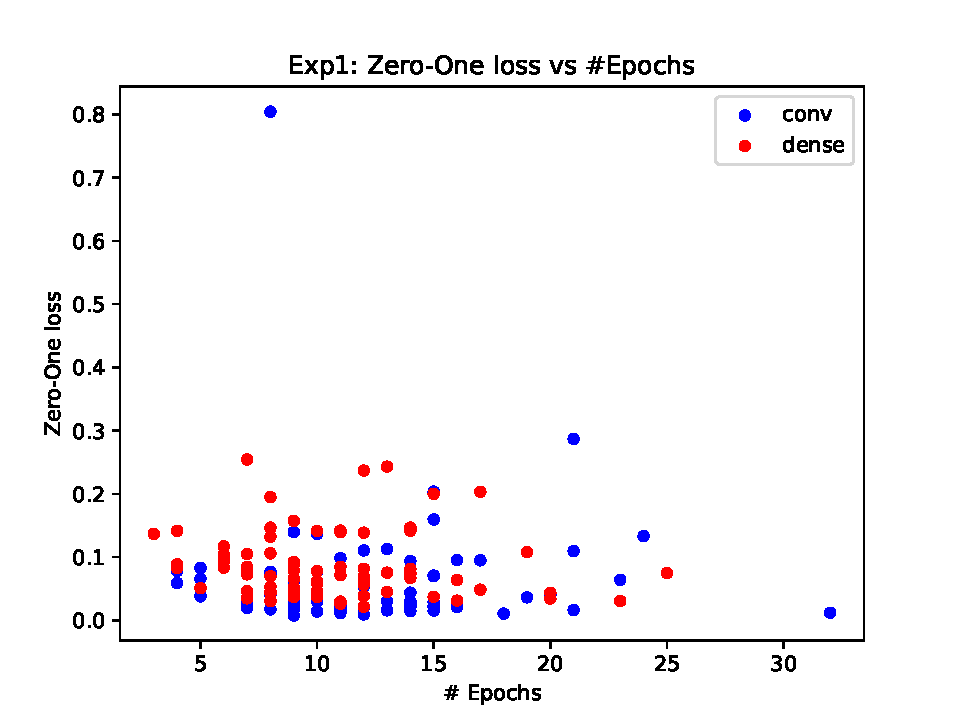
\includegraphics[width=\textwidth]{e1_loss_epochs}
\caption{Experiment 1: zero-one loss vs epochs}\label{fig:e1_loss_epochs}
\end{figure}

Figure\ref{fig:e1_40_loss_width} shows the zero-one loss achieved on images of size 40x40 pixels by ANNs of different depth and width, of type DNN and CNN respectively. The figures show that deeper and wider networks achieve a lower zero-one loss. Note that there is no overfitting in that data because the zero-one loss is computed on the testing set.
\begin{figure}
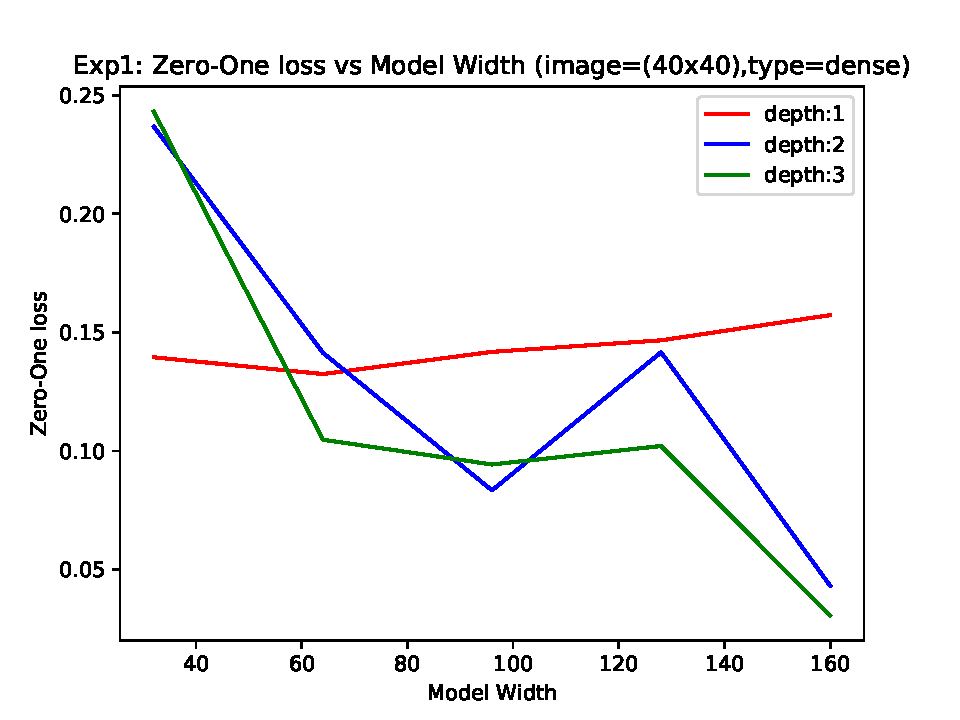
\includegraphics[width=\textwidth]{e1_40_dense_loss_width}
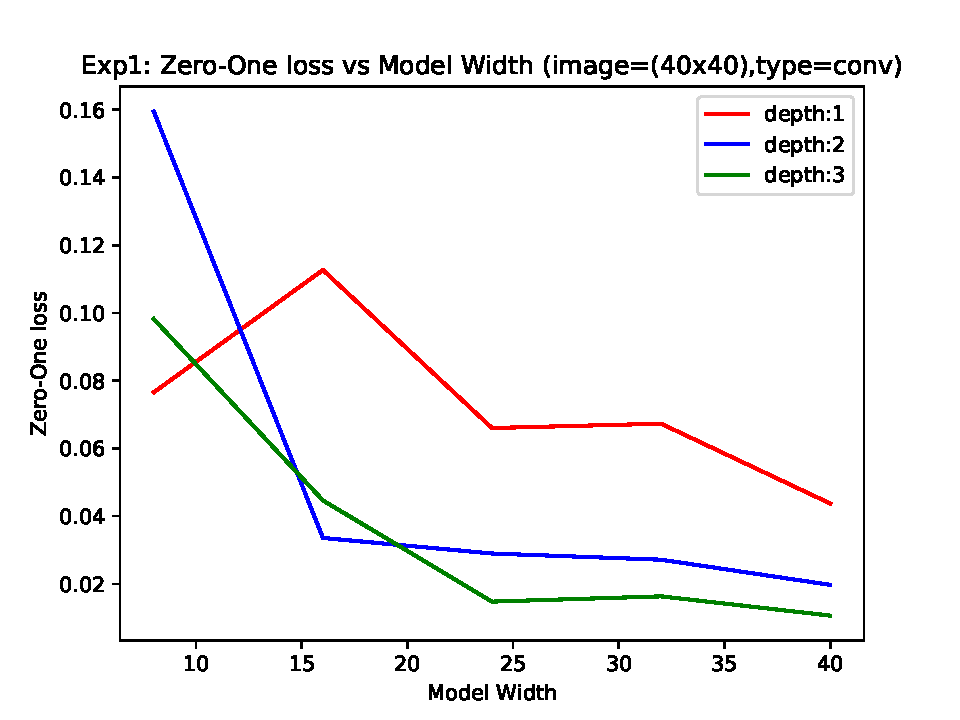
\includegraphics[width=\textwidth]{e1_40_conv_loss_width}
\caption{Experiment 1: zero-one loss vs ANN size}\label{fig:e1_40_loss_width}
\end{figure}

Results can be reproduced by following the steps highlighted in section\ref{sec:repro}.
